\section{ANALYSIS AND RESULTS}

In order to study the socio-technical congruence hypothesis for the Cargo package manager, I started analysing its package dependency network and the associated technical and social (commenting) activities of its GitHub contributors.
To do so, I focused on the three preliminary research questions presented in Section~\ref{sec:intro}.


\textbf{RQ1 - } How does the dependency network structure influence social activity? In this research question I am looking for any proof of relation between technical network structure and social interaction between contributors (E.g., are contributors more likely to be active in commenting on packages they depend on than on other packages?) in order to find an answer for this question I created a notebook containing a dependency network and contributors comment of different types and investiged temporal and structural relation between comment activity of developers and dependency network. 

\textbf{RQ2 - } How does the social activity of a contributor to a specific package increase his likelihood to start or stop depending on this package? As for this case I am looking for any kind of evidence showing that if there is any sort of relationship between social activity of the contributors of packages and temporal or structural pattern of dependency between packages. To do this in fact I basically tried to find a relation between any kind of social activity including issue comments, commit comment, pull review comment and pull comments of package maintainers and the dependency of each version of that package to find whether there is a tendency to put comment before start using a package or is there any behaviorial pattern between dependency network and social activity. If I can find any sign that shows its more likely for a developer to comment on package before start using it, based on this we can conclude social interaction can lead to technical dependency. My rudimental results shows that although not all activities will result in a technical dependency but there is priliminary evidence that shows there are a lot of cases that developer start using a package after commenting and to be more precise the result shows contributors tend to put comment on issues and pulls before depending on a package. the graph~\ref{fig:fig1} shows my finding in Cargo ecosystem.

\begin{figure}[htb]
    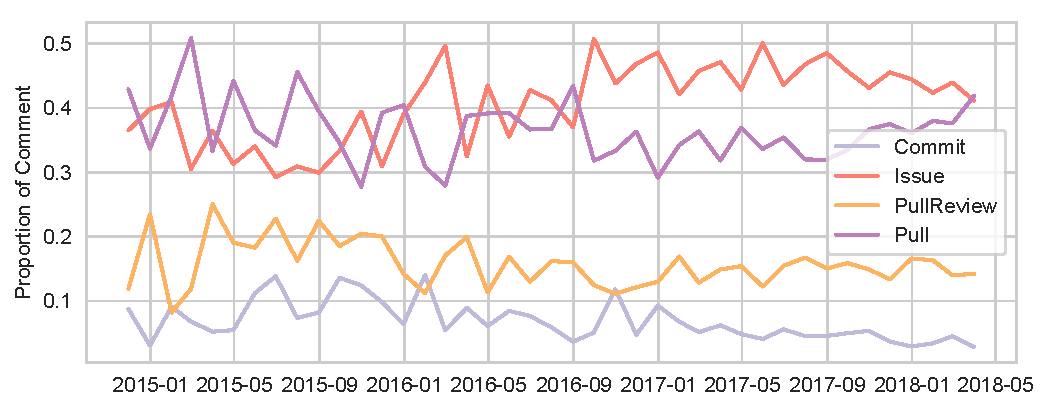
\includegraphics[width=\linewidth]{Photos/RQ22.pdf} 
    \caption{Proportion of comments on unique dependent packages before an after dependency}
    \label{fig:fig1}
\end{figure}


I also found that there are early signs of increase in commenting activity of developers before using a package as dependency and after june 2017 this trend has a drastic growth between contributors in Cargo ecosystem. the graph~\ref{fig:fig2} shows the emprical result of my investigations. 

\begin{figure}[thb]
    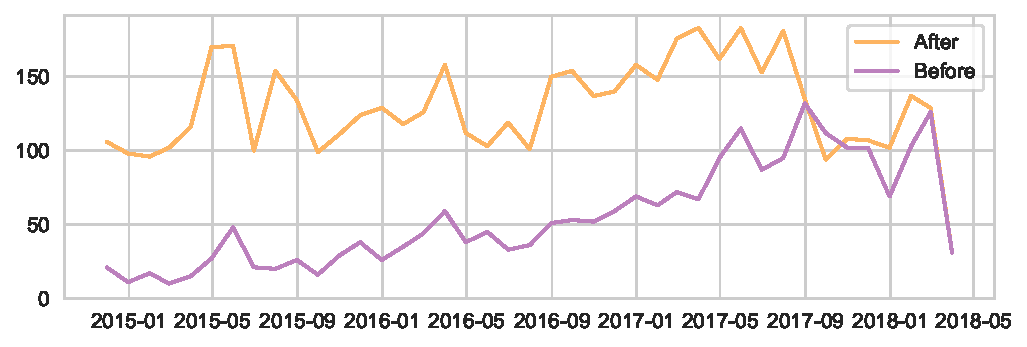
\includegraphics[width=\linewidth]{Photos/RQ21.pdf} 
    \caption{Number of packages with social activity of developer before start using it}
    \label{fig:fig2}
\end{figure}



\textbf{RQ3 - } How does the social activity of a contributor to a specific package increase his likelihood to start or stop becoming technically active for this package? The prerliminary result of my emprical study shows that package maintainers mostly start commenting on a issue before contributing to package. This shows that a contribution generally starts with an issue in some part of a package. the graph shows contributors tendency to comment before contributing to a package. 

\begin{figure}[thb]
    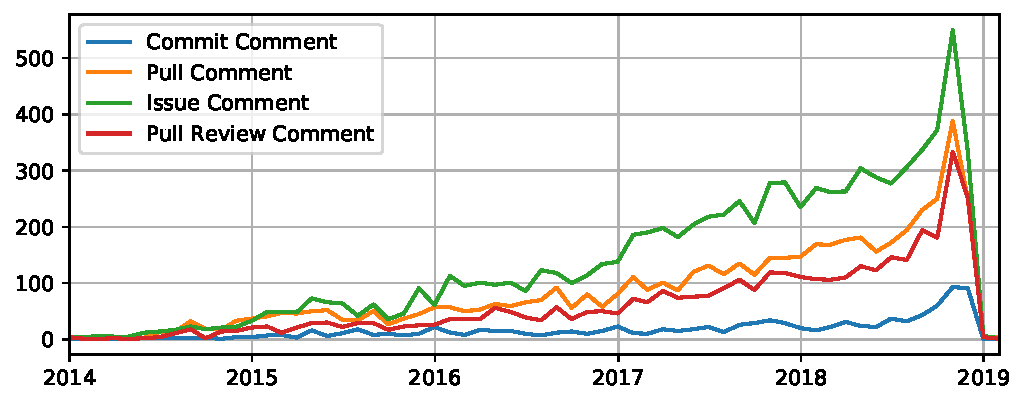
\includegraphics[width=\linewidth]{Photos/RQ3.pdf} 
    \caption{Comment avtivity before contributing to a package}
    \label{fig:fig3}
\end{figure}


